% $Header: /Users/joseph/Documents/LaTeX/beamer/solutions/generic-talks/generic-ornate-15min-45min.en.tex,v 90e850259b8b 2007/01/28 20:48:30 tantau $
\documentclass{beamer}

\mode<presentation>
{
  \usetheme{AnnArbor}
  % or ...

  \setbeamercovered{transparent}
  % or whatever (possibly just delete it)
}


\usepackage[english]{babel}

\usepackage[latin1]{inputenc}

\usepackage{times}
\usepackage[T1]{fontenc}
\usepackage[outdir=./]{epstopdf}
\usepackage{color,soul}

\newcommand{\source}[1]{\tiny \textcolor{gray}{Source: #1}}
\newcommand{\word}[1]{\texttt{#1}}
\newcommand{\wordvec}[1]{\textbf{v}[#1]}
\newcommand{\softmax}{\text{softmax}}
\newcommand{\cbow}{\text{CBOW}}
\newcommand{\skipgram}{\text{skipgram}}
\newcommand{\currentword}{{w_0}}
\newcommand{\context}{\mathcal{C}}
\newcommand{\vocabulary}{W}
\newcommand{\p}{P}
\newcommand{\crossentropy}{H}
\newcommand{\likelihood}{\mathcal L}
\newcommand{\correctoutput}{y}
\newcommand{\prediction}{\hat{y}}
\newcommand{\target}{y}
\newcommand{\sigmoid}{\sigma}
\newcommand{\transpose}[1]{#1^\top}
\newcommand{\smparam}{\beta}
\newcommand{\hsparam}{\theta}
\newcommand{\nsparam}{\gamma}

\title[Corpus Experiments]{Corpus Experiments for Word Embeddings}

%\subtitle
%{Presentation Subtitle} % (optional)

\author
{Benjamin Wilson (with Adriaan Schakel)}

\date[Berlin ML Learning Group] % (optional)
{Berlin ML Learning Group, July 28 2015}


\begin{document}
\graphicspath{{../outputs/}}

\begin{frame}
  \titlepage
\end{frame}

\begin{frame}{Outline}
  \tableofcontents
  % You might wish to add the option [pausesections]
\end{frame}

\section{Word Embeddings}

\begin{frame}{Word Embeddings}

\begin{itemize}
\item
associate words with points in space
\item
spatially encode word meaning and relationships between words
\item
learned from input texts
\item
e.g. word2vec, GloVe, ...
\end{itemize}

\end{frame}

\begin{frame}{Pictorially}
\begin{itemize}
\item spatial distance corresponds to word similarity
\item words are close together $\Leftrightarrow$ their "meanings" are similar
\end{itemize}
\begin{center}
    \includegraphics[height=140px]{semantic_similarity}\\
\end{center}
\end{frame}


\begin{frame}{Co-occurrence distributions}
\begin{itemize}
	\item Suppose we read the word $\word{cat}$.  What is the probability $\p ( w | \word{cat})$ that we'll read the word $w$ nearby?
\begin{center}
\includegraphics[height=30px]{dh}
\end{center}
\item $\p ( \cdot | \word{cat})$ is the \textit{co-occurrence distribution} of the word $\word{cat}$.
\item Distributional Hypothesis: the meaning of $\word{cat}$ is captured by the co-occurrence distribution.
\item Word embeddings are trained by sampling from the co-occurrence distribution.
\end{itemize}
\end{frame}

\section{Corpus Experimentalism}

\begin{frame}{Some Questions about Word Embeddings}
How would the word vector change if ...
\begin{enumerate}
	\item ... the word were less frequent? more frequent?
	\item ... the word were less informative? i.e. if $\p ( \cdot | \word{cat})$ were noisier? less noisy?
\end{enumerate}
\end{frame}

\begin{frame}{Different Approaches}
We could attempt to answer such questions by either:
\begin{enumerate}
	\item reasoning about the mechanism (\textbf{theoretical}).
	\item studying the data (\textbf{observational}).
	\item studying how the output changes when the input is varied in a controlled manner (\textbf{experimental}).
\end{enumerate}
\end{frame}

\section{Word Frequency Experiment}

\begin{frame}{Observing word frequency}
\begin{itemize}
	\item word frequency is encoded in vector length
		\begin{center}
		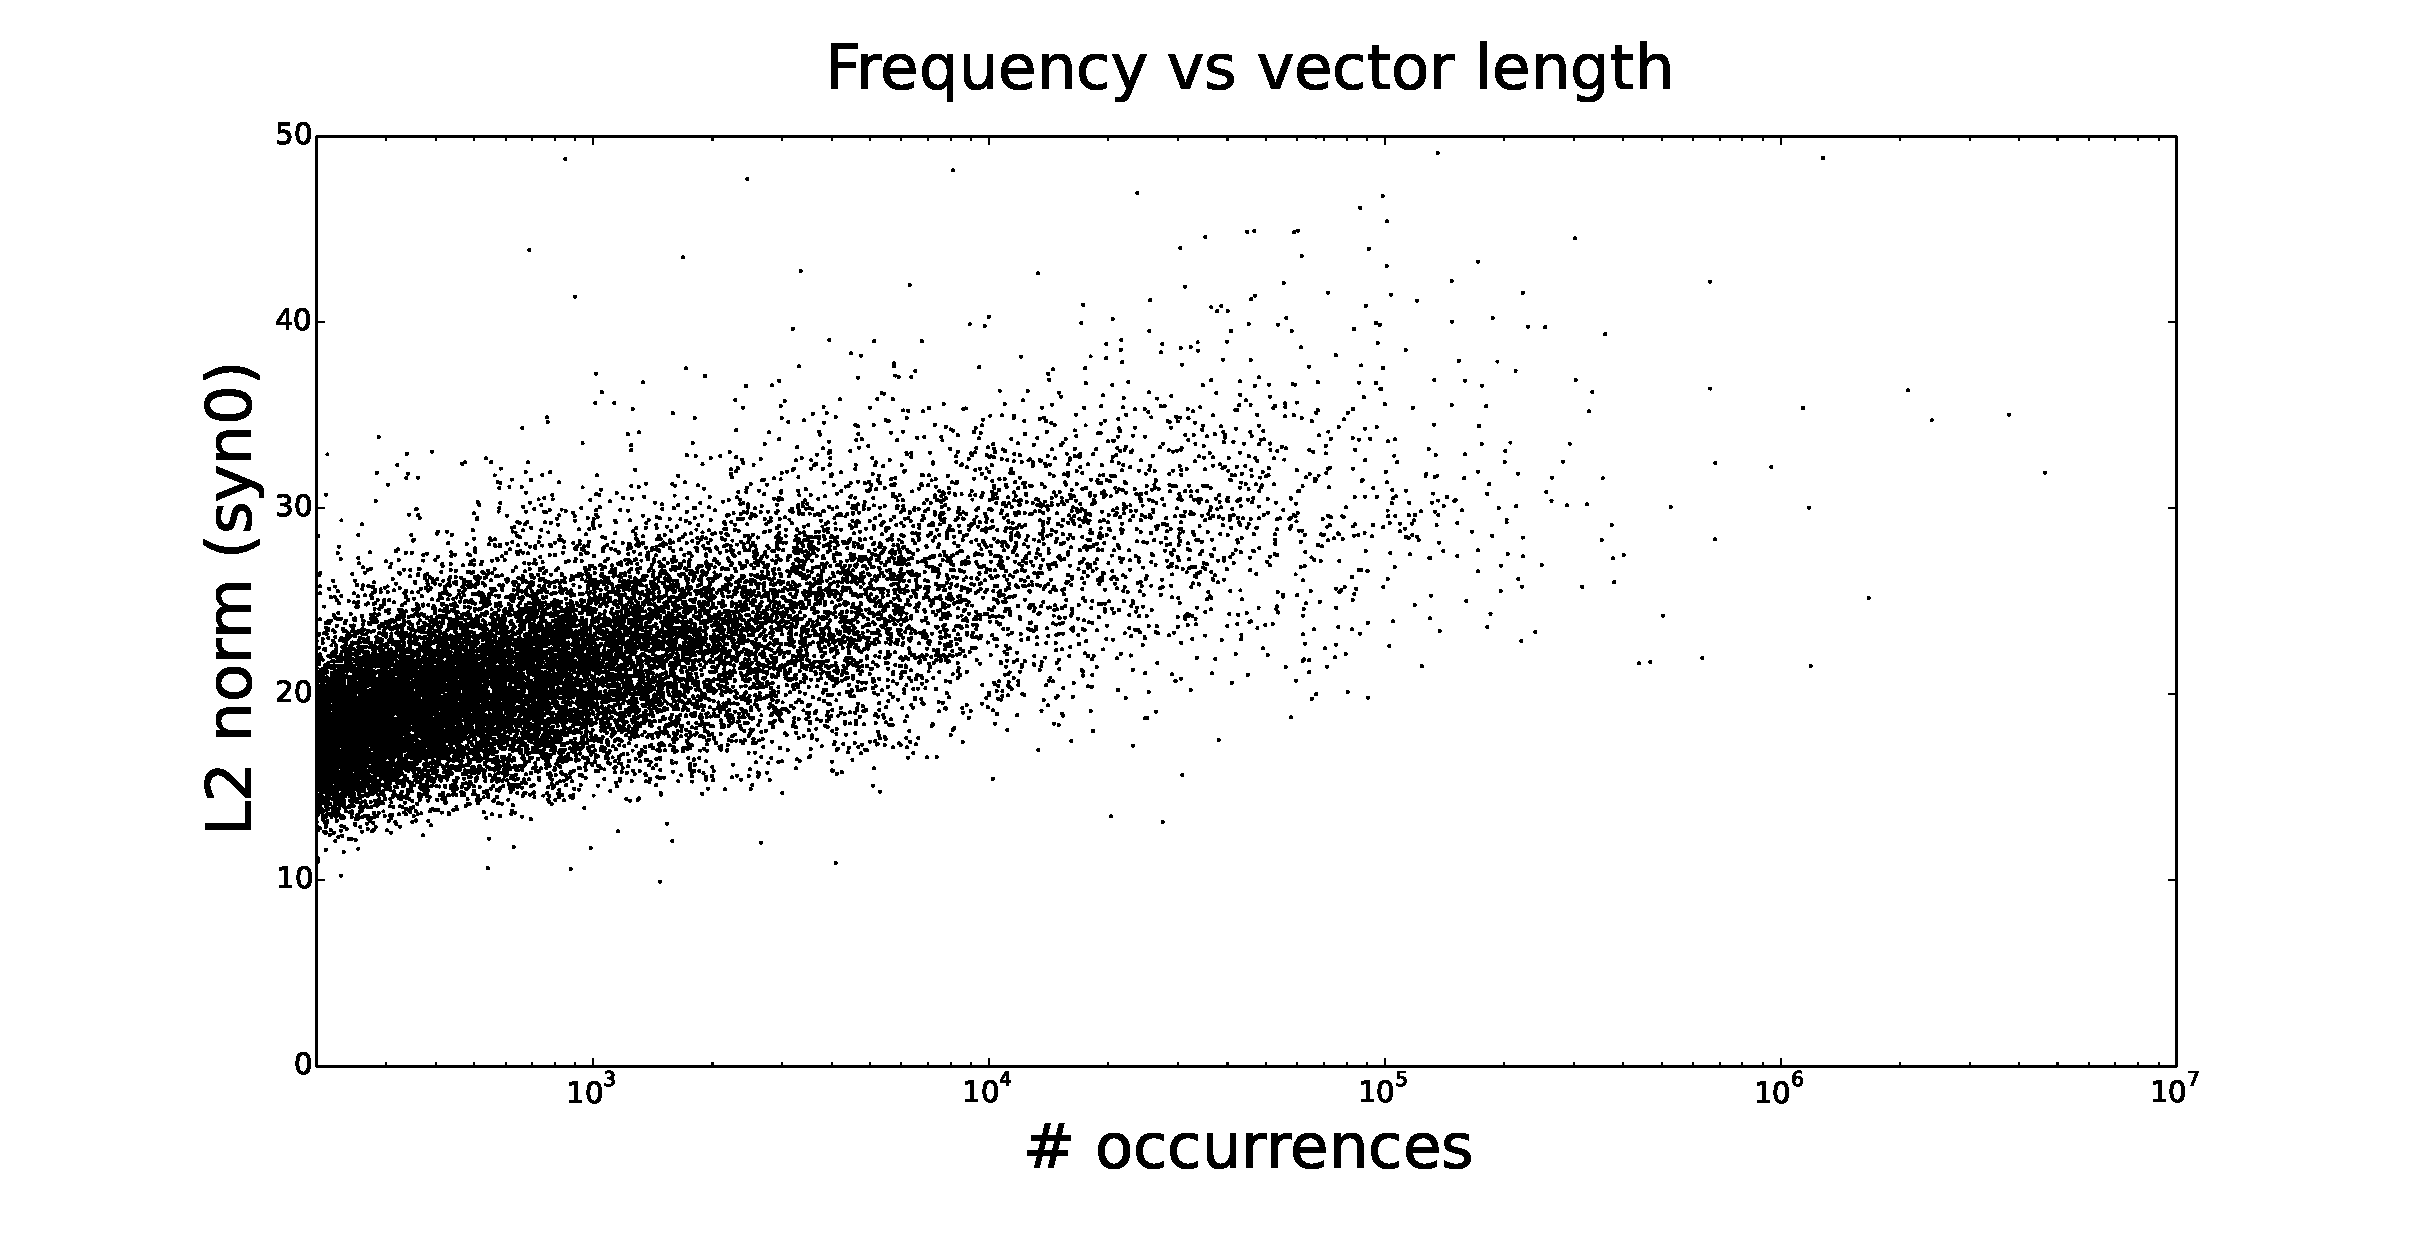
\includegraphics[height=80px]{frequency-norm-scatterplot} \\
		\end{center}
	\item but word frequency is related to many other things (e.g. significance)
	\item so difficult to determine \textbf{observationally} if vector length is related to word frequency \textbf{directly}
	\item for this, an experimental approach is required
\end{itemize}
\end{frame}

\begin{frame}{Word Frequency Experiment}
\begin{itemize}
	\item Modify the training corpus, replacing all occurrences of the word $\word{cat}$ with a token chosen from the distribution:
	\begin{center}
	\includegraphics[height=120px]{truncated-geometric-distribution} \\
	\end{center}
	\item Thus $\word{cat}$ is replaced by a family of tokens with varying frequencies, but the same co-occurrence distribution as $\word{cat}$.
	\item Train the word embedding on the modified corpus
	\item Study the word vectors of $\word{CAT\_i}$ for $i = 1, 2, \dots$.
\end{itemize}
\end{frame}

\begin{frame}{Word Frequency Experiment Example}
	\par
	{\small
\texttt{a pedigreed \textcolor{red}{CAT\_2} is one whose ancestry is recorded by a \textcolor{red}{CAT\_5} fancier organization
a purebred \textcolor{red}{CAT\_2} is one whose ancestry contains only individuals of the same breed
the semiferal \textcolor{red}{CAT\_1} a mostly outdoor \textcolor{red}{CAT\_1} is not owned by any one individual
the domestic \textcolor{red}{CAT\_1} was first classified as felis catus
the domesticated \textcolor{red}{CAT\_1} and its closest wild ancestor are both diploid organisms that possess  chromosomes and roughly  genes
...
dogs perform many roles for people such as hunting herding pulling loads protection assisting police and military companionship and more recently aiding handicapped individuals in  carl linnaeus listed among the types of quadrupeds familiar to him the latin word for dog canis among the species within this genus linnaeus listed the red fox as canis vulpes wolves canis lupus and the domestic dog canis canis in later editions linnaeus dropped canis canis and greatly expanded his list of the canis genus of quadrupeds and by  included alongside the foxes wolves and jackals and many more terms that are now listed as synonyms for domestic dog including aegyptius hairless dog aquaticus water dog and mustelinus literally badger dog among these were two that later experts have been widely used for domestic dogs as a species: canis domesticus and most predominantly canis familiaris the common or familiar dog} \par}
\end{frame}

\begin{frame}{Word Frequency Experiment Results (word2vec)}
	\begin{center}
	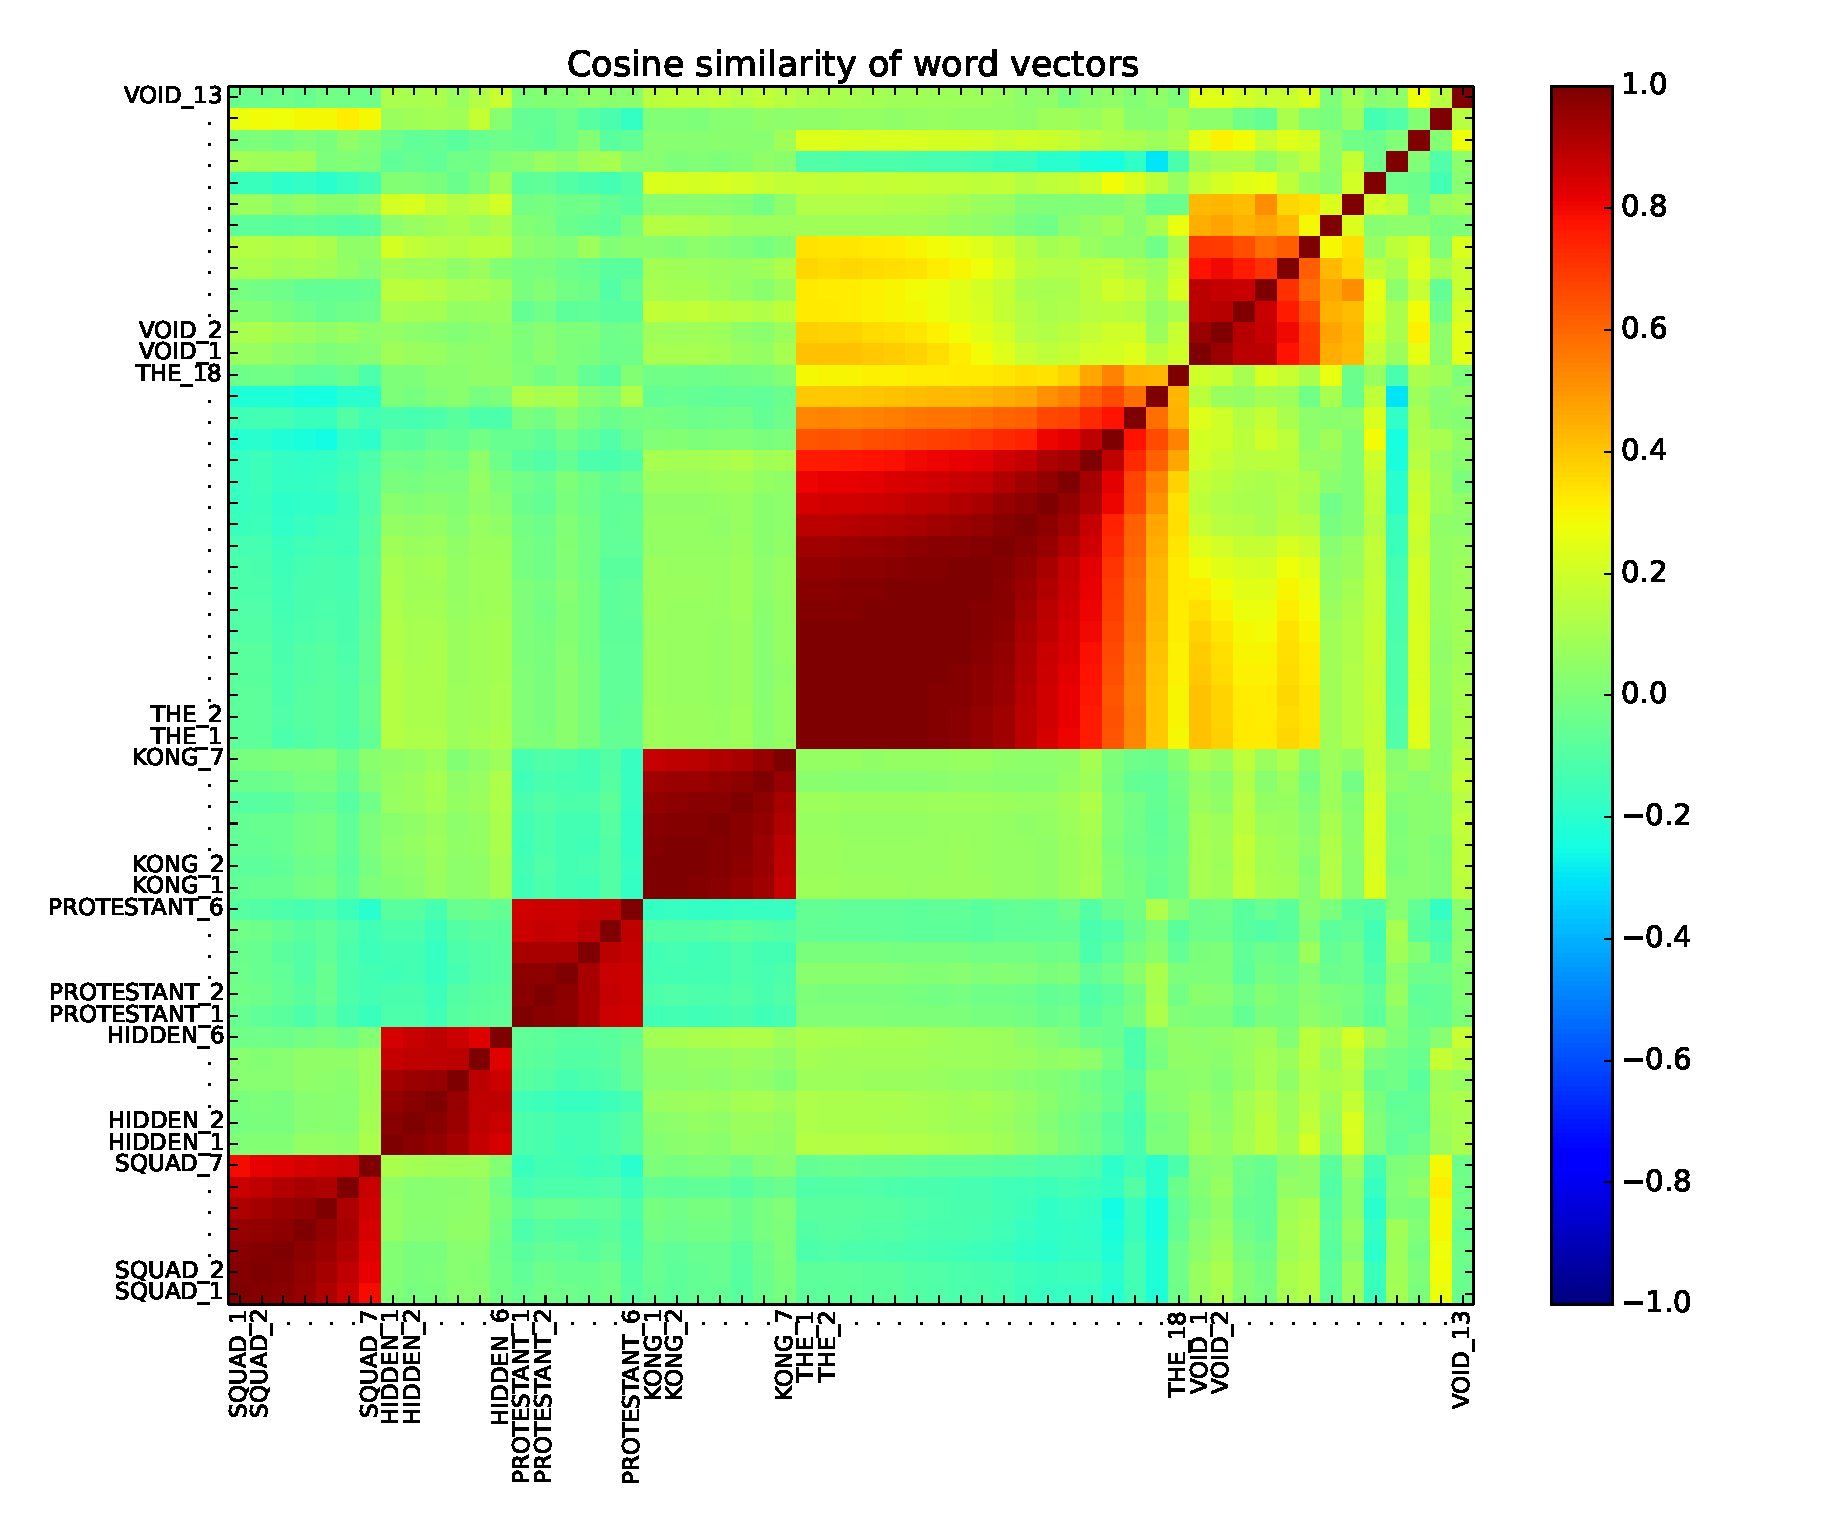
\includegraphics[height=200px]{word-frequency-experiment-heatmap} \\
	\end{center}
\end{frame}

\begin{frame}{Word Frequency Experiment Results (word2vec)}
	\begin{center}
	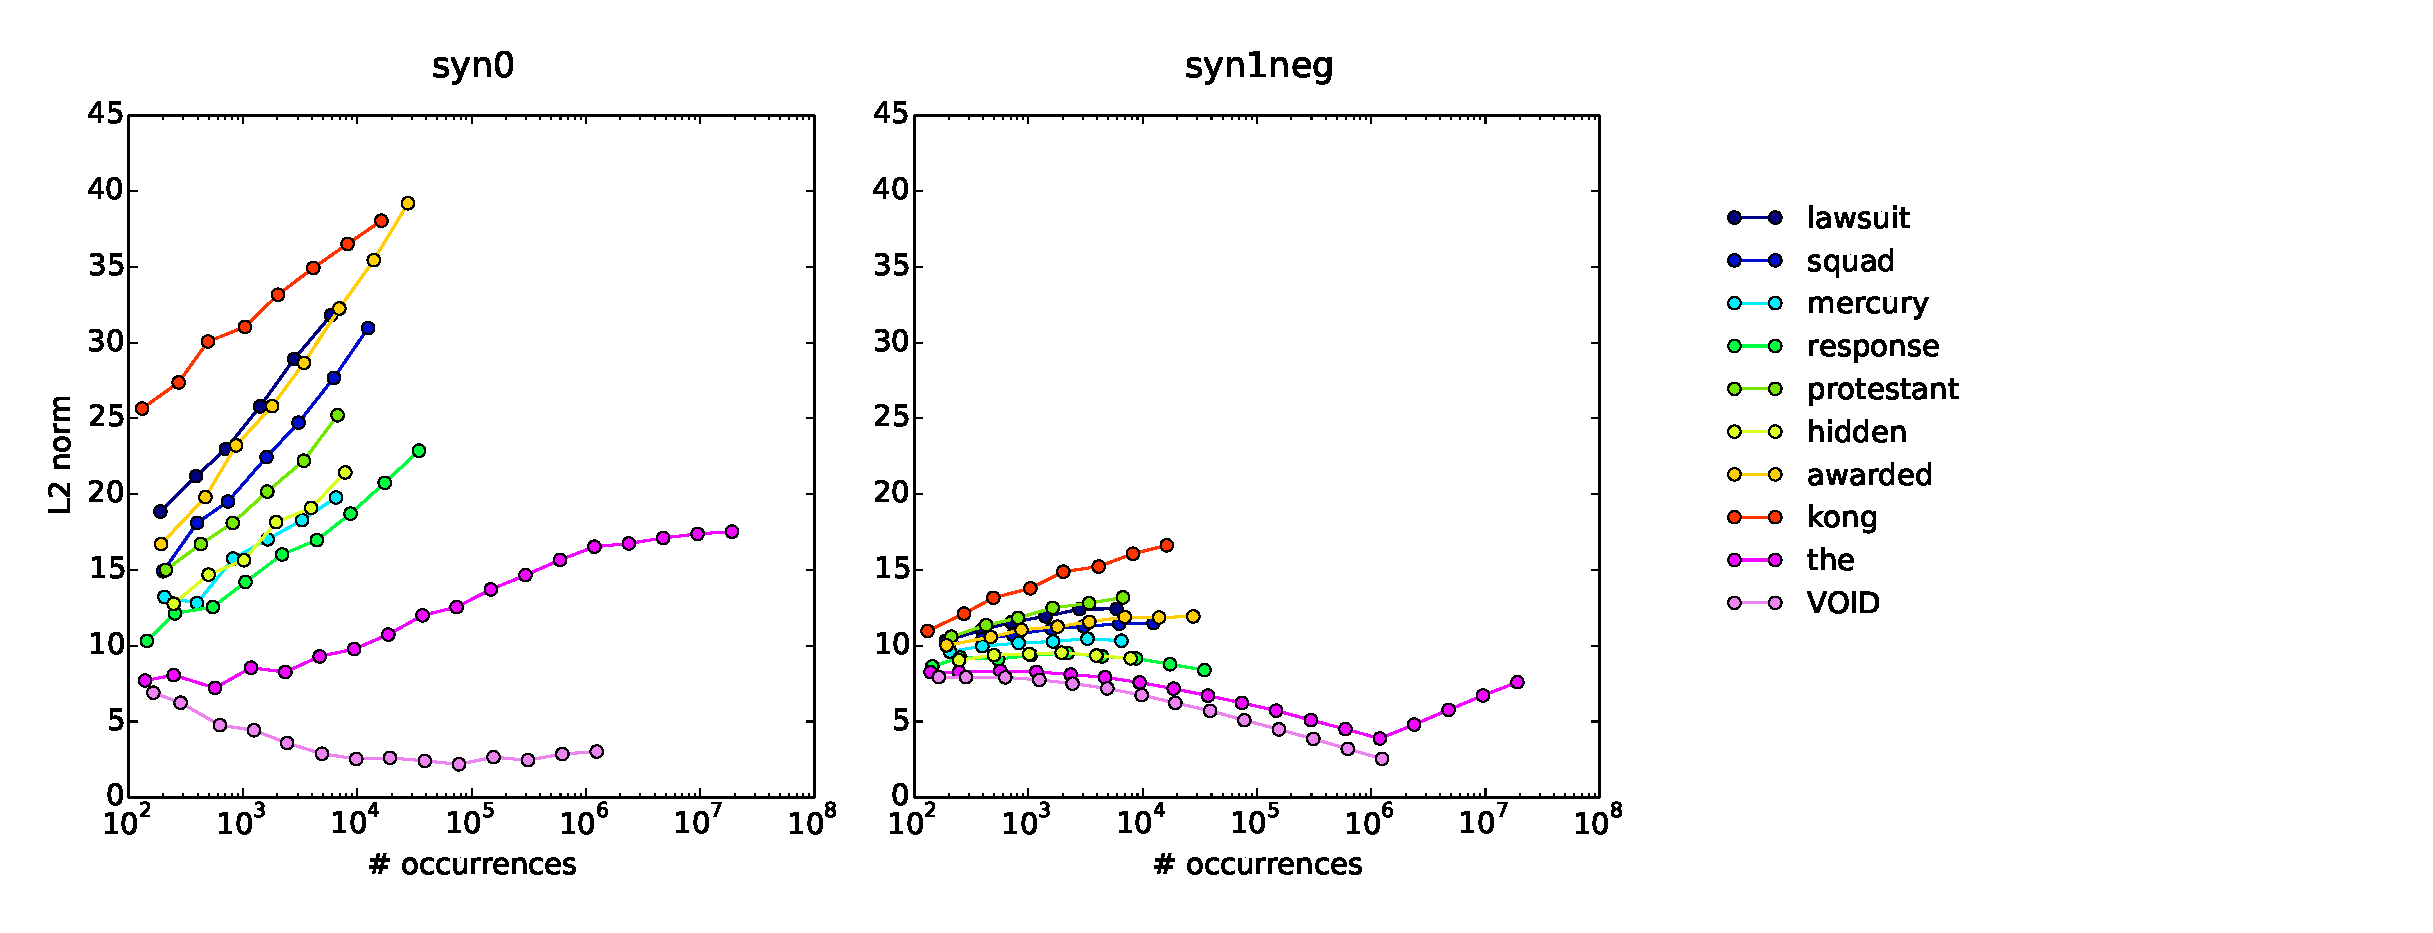
\includegraphics[height=150px]{word-frequency-experiment-graph} \\
	\end{center}
\end{frame}

\begin{frame}{Word Frequency Experiment Results (word2vec)}
	\begin{itemize}
		\item Vector direction is independent of frequency.
		\item Vector length depends directly and linearly on word frequency (for the word vectors, ``syn0'').
	\end{itemize}
\end{frame}

\section{Co-occurrence Noise Experiment}

\begin{frame}{Co-occurrence Noise Experiment}
\begin{itemize}
	\item Objective: vary the level of noise in the co-occurrence distribution, without varying the frequency.
	\item Our noise distribution is the global word frequency distibution.
	\item Thus we can introduce noise into the co-occurrence distribution of a word by randomly displacing some of its original occurrences throughout the corpus.
\end{itemize}
\end{frame}

\begin{frame}{Co-occurrence Noise Experiment Recipe}
How, exactly?
\begin{enumerate}
	\item Modify corpus as before, replacing the word $\word{cat}$ by tokens $\word{CAT\_i}$ for $i = 1, 2, \dots$ with varying frequencies.
	\item Introduce random occurrences of $\word{CAT\_i}$ into the corpus, such that its frequency is raised to that of $\word{cat}$.
\end{enumerate}
\end{frame}

\begin{frame}{Co-occurrence Noise Experiment Example}
	\par
	{\small
		\texttt{ a pedigreed \textcolor{red}{CAT\_1} is \textcolor{red}{\textit{CAT\_3}} one whose ancestry is recorded by a \textcolor{red}{CAT\_1} fancier organization
a purebred \textcolor{red}{CAT\_3} is one whose ancestry contains only individuals of the same breed
the semiferal \textcolor{red}{CAT\_2} a mostly outdoor \textcolor{red}{CAT\_2} is not owned by any one individual
\textcolor{red}{\textit{CAT\_2}} the domestic \textcolor{red}{CAT\_3} was first classified as felis catus
the domesticated \textcolor{red}{CAT\_1} and its closest wild ancestor are both diploid organisms \textcolor{red}{\textit{CAT\_3}} that possess  chromosomes and roughly  genes
...
the domestic dog canis lupus familiaris or canis familiaris is a domesticated canid which has been selectively bred for millennia for various behaviors sensory capabilities and physical attributes
although initially thought to have originated as a manmade variant of an extant canid species variously supposed as being the \textcolor{red}{\textit{CAT\_1}} dhole golden jackal or gray wolf \textcolor{red}{\textit{CAT\_3}} extensive genetic studies undertaken during the s indicate that dogs \textcolor{red}{\textit{CAT\_2}} diverged from a now-extinct canid in eurasia
} \par}
\end{frame}

\begin{frame}{Co-occurrence Noise Experiment Results (word2vec)}
	\begin{center}
	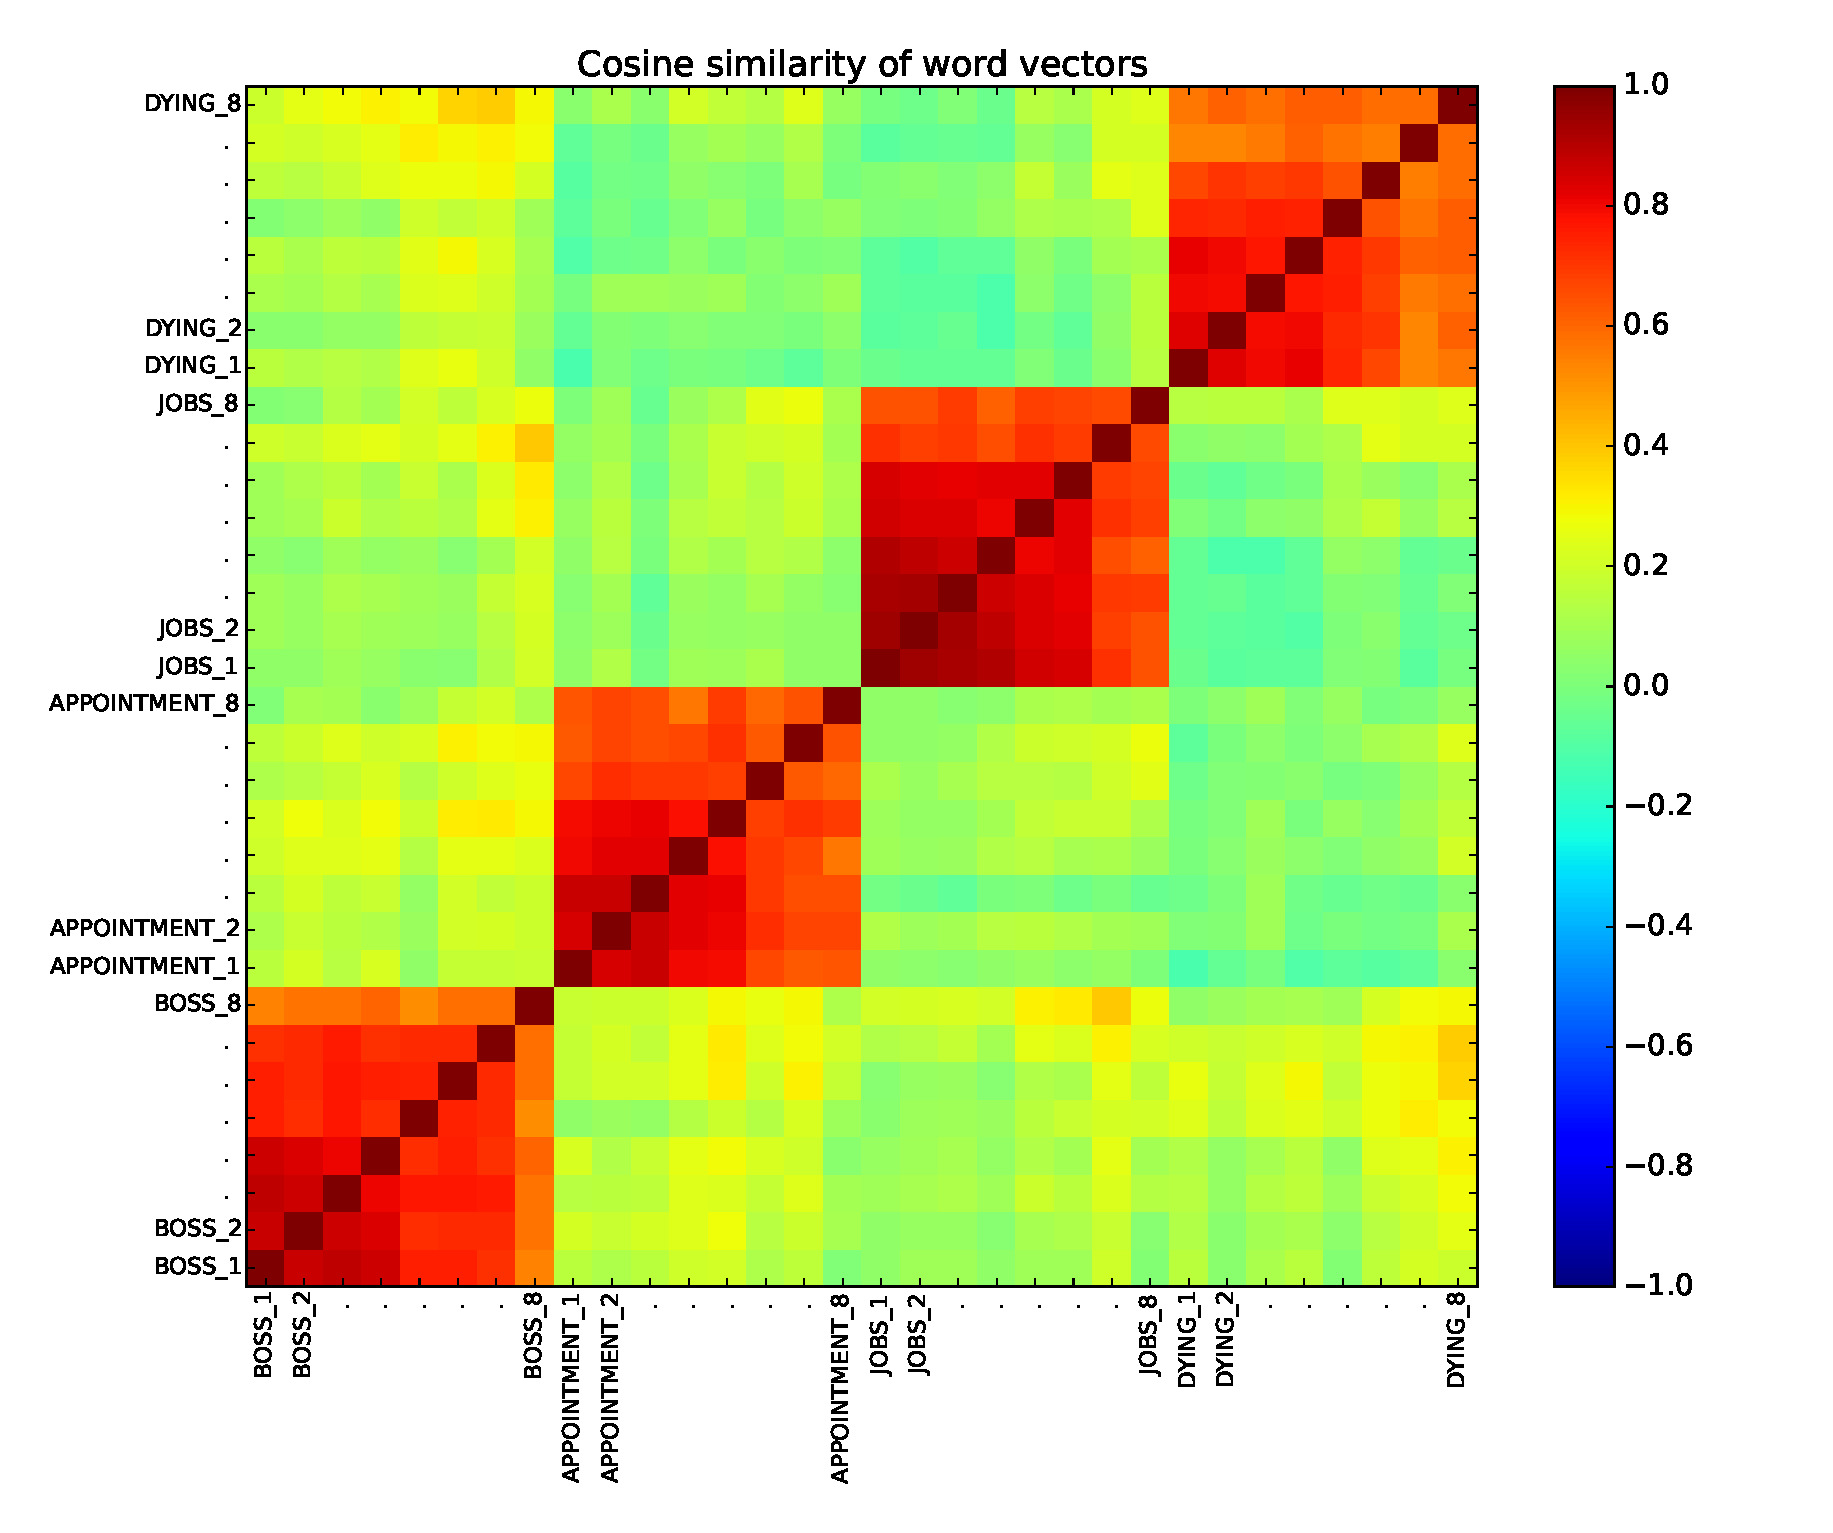
\includegraphics[height=200px]{cooccurrence-noise-heatmap} \\
	\end{center}
\end{frame}


\begin{frame}{Co-occurrence Noise Experiment Results (word2vec)}
	\begin{center}
	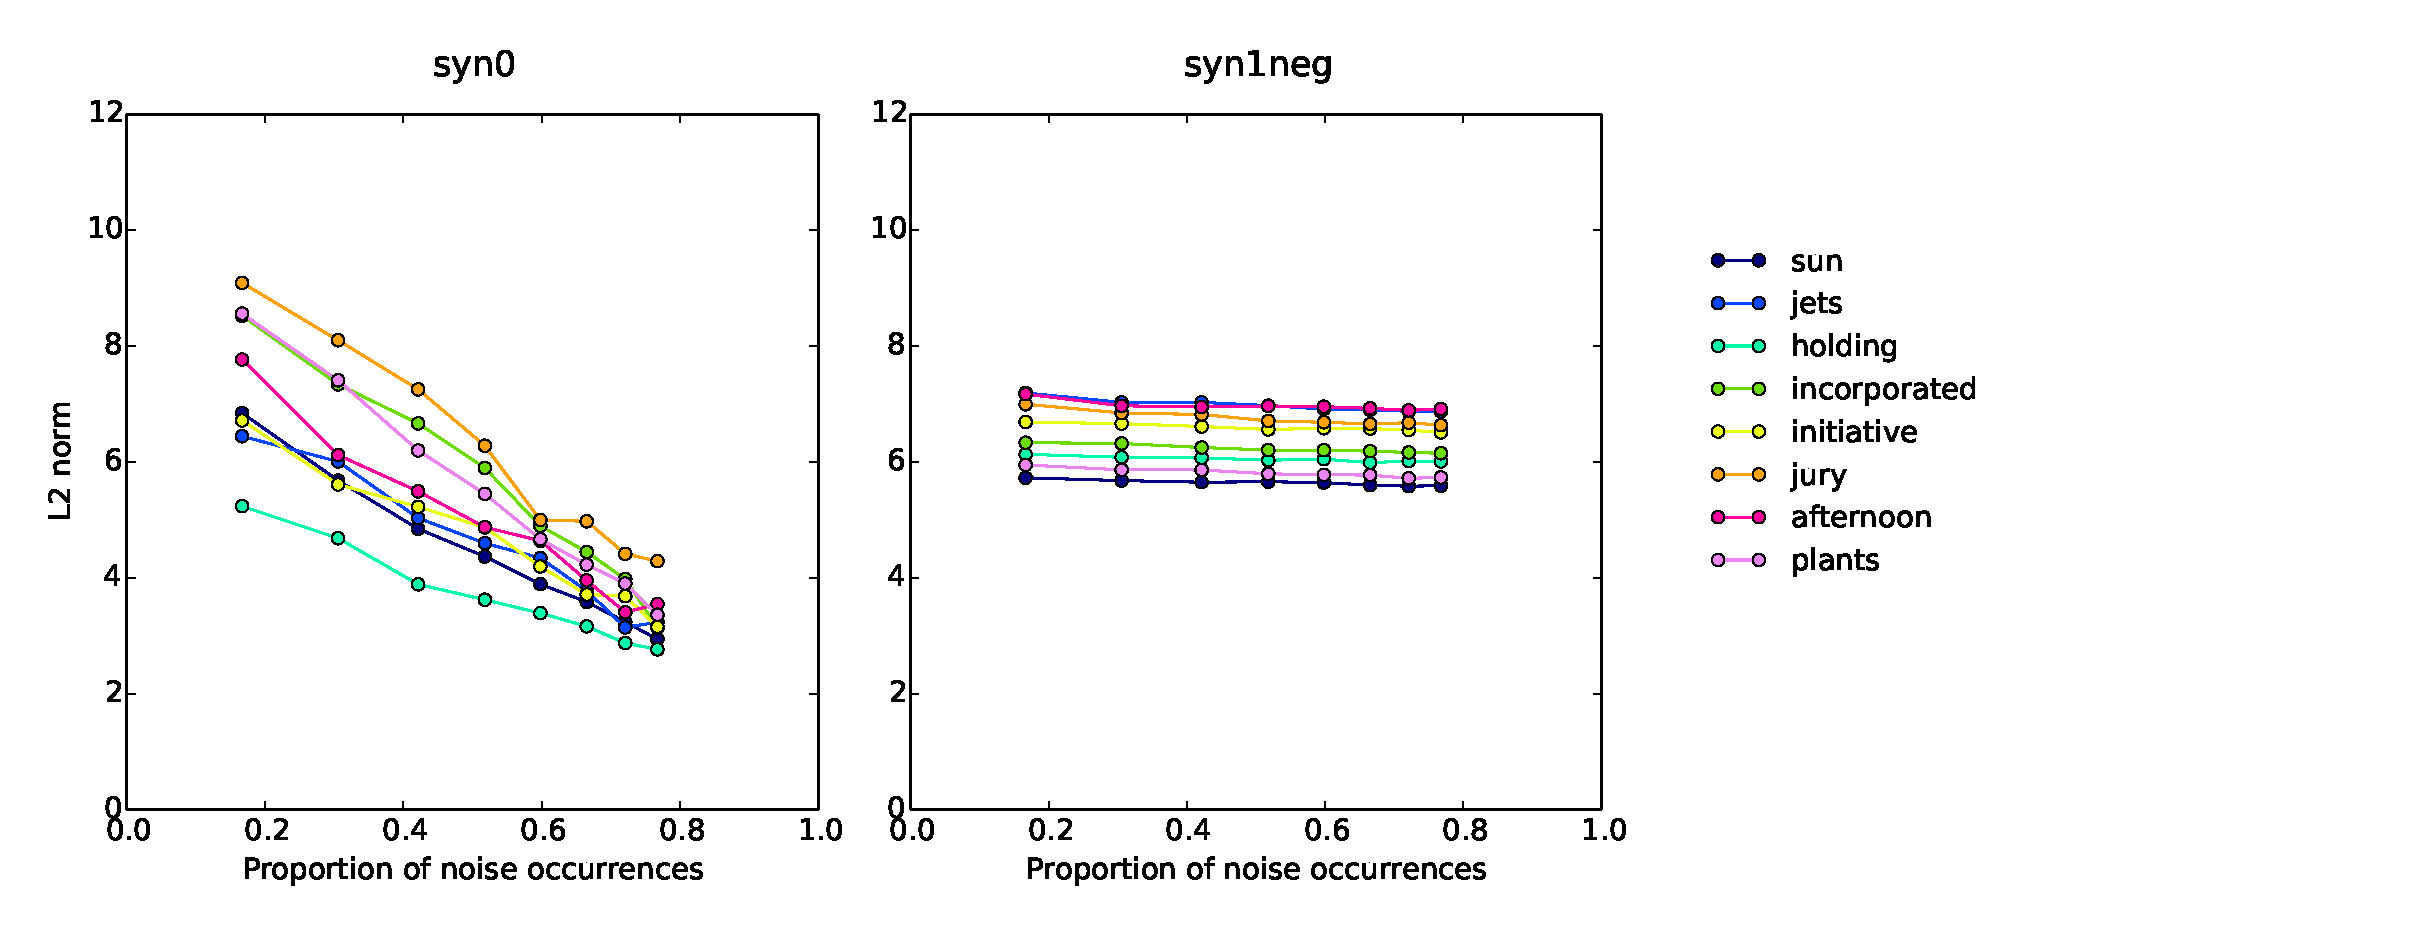
\includegraphics[height=150px]{cooccurrence-noise-graph} \\
	\end{center}
\end{frame}

\begin{frame}{Co-occurrence Noise Experiment Results (word2vec)}
	\begin{itemize}
		\item Vector direction is remarkably insensitive to co-occurrence noise.
		\item Vector length depends directly, linearly, on the level of co-occurrence noise.
		\item This suggests that, within any frequency band, vector length can be taken as a measure of signal strength.
	\end{itemize}
\end{frame}

\section{Appendix: word2vec}
\begin{frame}{Learning from text}
\begin{itemize}
\item word2vec learns from input text
\item considers each word \textcolor{red}{$\currentword$} in turn, along with its context \textcolor{red}{$\context$}
\item context = neighbouring words (here, for simplicity, 2 words forward and back)
\begin{center}
\includegraphics[height=45px]{context} \\
\vspace{0.5cm}
\begin{tabular}{c | c | c}
sample \# & $\currentword$ & context $\context$ \\ \hline
	1 & \word{once} & \{\word{upon}, \word{a}\} \\
 & $\cdots$ &  \\
4 & \word{time} & \{\word{upon}, \word{a}, \word{in}, \word{a}\} \\
 & $\cdots$ &  
\end{tabular}

\end{center}
\end{itemize}
\end{frame}

\begin{frame}{Two approaches: CBOW and Skip-gram}
word2vec can learn the word vectors via two distinct learning tasks, \textcolor{red}{CBOW} and \textcolor{red}{Skip-gram}.
\begin{itemize}
\item CBOW: predict the current word $\currentword$ given only $\context$
\item Skip-gram: predict words from $\context$ given $\currentword$
\item Skip-gram produces better word vectors for infrequent words
\item CBOW is faster by a factor of window size -- more appropriate for larger corpora
\item We will speak only of CBOW (life is short).
\end{itemize}
\end{frame}

\begin{frame}{CBOW learning task}
\begin{itemize}
	\item Given only the current context $\context$, e.g. $$\context = \{\word{upon}, \word{a}, \word{in}, \word{a}\}$$   predict which of all possible words is the current word $\currentword$, e.g. $\currentword =$ \word{time}.
	\item multiclass classification on the vocabulary $\textcolor{red}{\vocabulary}$
	\item output is $\textcolor{red}{\prediction} = \prediction (\context) = \p ( \cdot | \context)$ is a probability distribution on $\vocabulary$, e.g.
		\begin{center}
			\includegraphics[height=40px]{prediction}
		\end{center}
	\item train so that $\prediction$ approximates target distribution $\textcolor{red}{\target}$ -- ``one-hot'' on the current word, e.g.
		\begin{center}
			\includegraphics[height=40px]{target}
		\end{center}
\end{itemize}
\end{frame}

\begin{frame}{Training CBOW with softmax regression}
	\textbf{Model}: $$\prediction = \p ( \cdot | \context ; \alpha, \smparam) = \softmax_\smparam (\sum_{w \in \context} \alpha_w), $$ where $\alpha$, $\smparam$ are families of parameter vectors.  Pictorially:
\begin{center}
\includegraphics[height=130px]{cbow}
\end{center}
In practice, hierarchical softmax or negative sampling is used in place of softmax.
\end{frame}

\begin{frame}{Stochastic Gradient Descent}
\begin{itemize}
\item learn the model parameters (here, the linear transforms)
\item minimize the difference between output distribution $\prediction$ and target distribution $\target$, measured using the cross-entropy $\textcolor{red}{\crossentropy}$:
	$$ \crossentropy (\target, \prediction) = - \sum_{w \in \vocabulary} \target_w \log \prediction_w $$
\item given $\target$ is one-hot, same as maximizing the probability of the correct outcome 
	$$\prediction_\currentword = \p (\currentword | \context ; \alpha, \smparam).$$
\item use stochastic gradient descent: for each (current word, context) pair, update all the parameters once.
\end{itemize}
\end{frame}

\begin{frame}{Word Representation}
\textit{Post-training}, associate every word $w \in \vocabulary$ with a vector $\wordvec w$:
\begin{itemize}
\item $\wordvec w$ is the vector of synaptic strengthes connecting the input layer unit $w$ to the hidden layer
\item more meaningfully, $\wordvec w$ is the hidden-layer representation of the single-word context $\context = \{w\}$.
\item vectors are (artifically) normed to unit length (Euclidean norm), post-training.
\end{itemize}
\end{frame}

\end{document}


